\section{Interface Design}
The interface for this application is designed to look like other social media, due to the fact that this makes it easier for
 new users, as they will know what the various buttons and tabs do from previous experience. The overall design looks like this:
\clearpage
\noindent\makebox[\textwidth]{
\begin{tabularx}{1.5\textwidth} {XX}
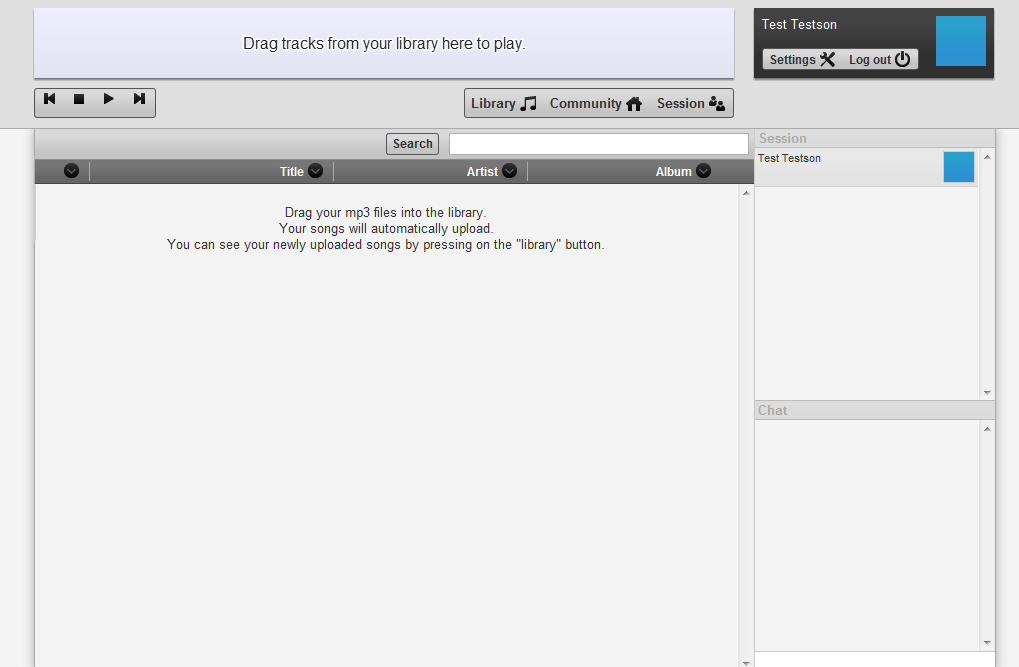
\includegraphics[scale = 0.6]{design/figures/general_interface}
\end{tabularx}}
The musicplayer, the box with settings and name of the person logged in and the two sidebars with session and chat are always
visible, seeing as these represent the most important aspects of the application: playing music and joining sessions with
other people. 

\vspace{10pt}
The buttons that change between the Library, Community and Session tabs are also always visible, seeing as
these represent the main navigation in the application. The icons used to represent these, are chosen to show, what their
fuction is, e.g. the note represents the music library, the house represents the home of the social life of the page in the
community tab and the two people in the session tab shows that this is where actual interaction happen. The buttons change
colour to indicate which tab is currently being viewed. 

\vspace{10pt}
The Settings button has a wrench and screwdrive to indicate that this
is where one should change settings. Pressing the Settings button opens a popup with the current information, giving the user the option to change it.

\vspace{10pt}
The tab that is open, is an empty library. The text on the page reads: ``Drag your mp3 files here to upload. Your songs will
automatically upload. You can see your newly uploaded songs by pressing the ``library'' button.'' This text is to inform the
user, that the upload method for this application is drag and drop, which might be new to some users. The music player,
unless it is playing music, displays the text: ``Drag tracks from your library here to play'.', to tell the user that
playback is also drag and drop. 

\vspace{10pt}
The session sidebar shows the people that you are currently in a session with, and the chat sidebar below shows chat between
people in the session.

Below is a screenshot of the community interface:

\noindent\makebox[\textwidth]{
\begin{tabularx}{1.5\textwidth} {XX}
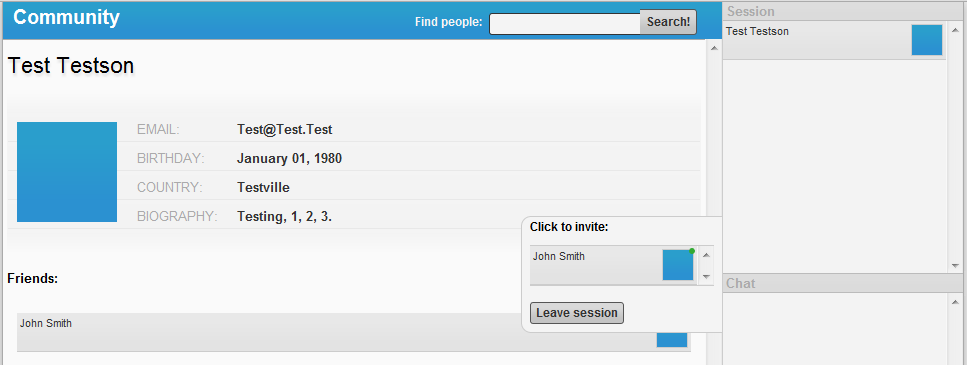
\includegraphics[scale = 0.69]{design/figures/community}
\end{tabularx}}
This shows the profile of the person Test Testson. All information is visible to friends of Test Testson, and can be changed
by him. The e-mail shown is not necessarily the one used to register with, although it is at first. This is the info, that has
so far been deemed relevant to a social webpage, to give other users a chance to get to know Test Testson before requesting
friendship with him. 

Under the information is a list of Test Testson's friends, which currently contains a list of online
friends, with one friend: John Smith. In case Test Testson gets any new friend requests, these will show up as a button on the profile of Test Testson which can be clicked to either accept or reject the person requesting friendship. This is similar to
other social webpages, which should give the user an instant understanding of how the friendship functionality works. 

\vspace{10pt}
Should test desire to invite people to a session, he can do so in the little flyout visible in the above picture. It flies out when mousing over the session sidebar, and give the user the option to invite online friends to a session.

\vspace{10pt}
The Session tab shows invites to sessions. This is a very simple page on which the user can accept or reject invitations, and as such is not shown with a screenshot. 